\documentclass[a4paper,10pt]{article}
\usepackage[utf8]{inputenc}
\usepackage{url}
\usepackage{enumerate}
\usepackage{verbatim}
\usepackage{graphicx}
\usepackage{changepage}% http://ctan.org/pkg/changepage
\usepackage{lipsum}% http://ctan.org/pkg/lipsum
\graphicspath{ {images/} }

%paragraph indentation
\setlength{\parindent}{4em} 

%paragraph spacing
\setlength{\parskip}{1em}

%Line spacing
% \renewcommand{\baselinestretch}{1.5}


\title{ \textbf{Study and Implementation of SDS\\ Independent-study report}}

\author{ Supervisor - Prof. S C Gupta \\
Aashish Goyal (2012CS10202) \\
Devansh Dalal (2012CS10224)  }

\begin{document}

\maketitle

\abstract{This study aims to understand the relevance of software defined storage systems(SDS), which is the current state of the art in storage solutions. The study shall look at the shortcomings of older distributed storage solutions, the essential components of sds and how it addresses the shortcomings. Then it dives in to give an overview of the architecture of an open source solution -- Ceph. Finally it concludes by documenting our efforts to set up a virtual cluster using ceph and proposes scenarios in which the department may put the ceph cluster to use. }    

\section{Introduction}
    SDS may be defined as a data storage method in which management and functioning of the data is abstracted from the actual physical storage and is controlled by software. The aim is create a system that can handle petabytes of data, simplify the complexity associated with managing such a system, provide fault tolerance and self healing capabilities. As the size and performance requirements of storage systems have increased, file system designers have looked to new architectures to facilitate system scalability. The emerging object-based storage paradigm diverges from commonly used server based architectures and forms the heart of many of the SDS systems currently in use. First let us try to define a bit more precisely what a storage system needs to offer in order to qualify as a SDS solution. Then we shall look at older storage distributions and understand their limitations which ultimately led to this new paradigm.
    
\section{Components of SDS}
SDS is part of the SDDC (Software Defined Data Center) vision that extends virtualization concepts such as abstraction, pooling, and automation to all of the data center’s resources and services. Compute infrastructure was the first to shift from monolithic mainframe systems running a handful of applications to x86-based commodity hardware and was then followed by network infrastructure. While it is understood that SDS involves virtualization of storage resources, there is no standard accepted definition as to what this refers to. Here we look at a list of essential components, compiled by referring several definitions of SDS, that storage system must possess to qualify as a software defined storage.

\begin{enumerate}[1]

    \item  \textbf{\texttt{Abstraction }}  The storage resources are virtualized and presented to the control plane where they can be configured as needed
    
    \item  \textbf{\texttt{Commodity Hardware }} These should be able to use easily available commodity hardware for storage as well as network needs. This leads to much lower operation costs compared to traditional solutions.
    
    \item  \textbf{\texttt{Automation}} Should provide automation to provide policy-based provisioning of storage. The user need not dive into the inner details of physical configuration of drives when needing space, say for some application.  
    
    \item  \textbf{\texttt{Resource Pooling }} The storage resources are pooled into a single logical entity and managed centrally by the control plane. 
    
    \item  \textbf{\texttt{Elasticity }} It should be possible to add/remove storage devices from the cluster and also change the allocation of space to the user on the fly.
    
    \item  \textbf{\texttt{Management Simplicity }} It is imperative that the system is easy to manage so that the skill and labour needed for implementing SDS is less.
\end{enumerate}



\newpage
\section{Traditional Storage Solutions}

As we are considering architectures for dealing with large amounts of data accessed simultaneously by several users, local file systems rarely fit the bill. The desire to share storage resources and data in networked computing environments has given rise to a number of client-server file systems. Common solutions in this space are NFS and CIFS, wherein a central server is allowed to export a local file system to remote systems who can then map it into their own namespace and provide access to the user. This centralized storage lead to the creation of high performance storage systems, of which NAS – Network Attached Storage is the most popular one. Network-attached storage (NAS) is a file-level computer data storage server connected to a computer network providing data access to a heterogeneous group of clients – a specialized computer built from the ground up for storing and serving files connected over the network. However the centralization present in the client server architecture has proven to be a bottleneck to scalability. 

The other paradigm which is popular are the distributed  file systems. They were designed to attempt to address the fundamental load balancing and scaling challenges inherent in client-server systems. These utilize a central server to coordinate file system access, and issue leases to explicitly promise the validity of data (or metadata) provided to the client cache for a specified period. SAN file systems belong to this cateogory of file-systems. A storage area network (SAN) is a dedicated network that provides access to consolidated, block level data storage on which a file system can be mounted. However such systems occasionally do not conform to the POSIX standard and already complicated enough when used along with a file system. Scaling them to petabytes is thus not considered practical.

Moreover the functionality of legacy file systems such as appending, amending files, permissions etc. are not a good fit to today’s use case. Most of the data that is currently being generated is unstructured and immutable .These features then only add to complexity, greater overhead and lot of meta-data management. Further the directory based structure of file-system which despite being extremely intuitive and useful also adds up to the complexity of locating the file in a file-system and is a poor fit for the REST API which is common today for accessing data in the cloud. RAID, the de-facto scheme for data protection also fails to scale. The scheme works well in small drives but as the data size increases the time to recover also increases. Long down-times are not acceptable by today’s standards and hence alternatives such as replication or erasure coding need to be adopted. 

\newpage    
\section{Object Storage}
    This is a storage architecture which manages data as objects rather than file systems which manage data as files in a hierarchy. The objects include the data, some associated meta-data and a uid (unique identifier) to search and access them. In case of updates to the data the entire object is replaced. Although this may seem as expensive and lacking in features at first, it turns out that the simplicity offered by such an organization of data makes it very easy to scale and manage. Further current usage pattern on data involves vast amount of immutable data and hence this pattern is also a good fit here. The meta-data in this case is associated with the object (not the file-system) and hence does not pose a barrier to scalability. Object storage is one of the most sought after features in modern storage systems. In such systems, \verb|I/O| instead of acting on small fixed sized blocks occurs on variable size objects. In such cases certain functionality such as low level block allocation decisions, security enforcement can be distributed to the device itself. This reduces burden on the servers managing meta data and helps the system to scale.
    

\newpage
\section{Architecture Of Hadoop File System}

Hadoop file system\cite{borthakur2008hdfs} is a distributed file system designed to meet the needs of very large storage systems. It introduces several of the ideas upon which Ceph is designed and thus is considered here as logical pre cursor before introducing Ceph itself. It was designed keeping in mind the folowing goals and assumptions
\begin{enumerate}[1]

    \item  \textbf{\texttt{Hardware Failure }}  
    
    \item  \textbf{\texttt{Commodity Hardware }} 
    
    \item  \textbf{\texttt{Streaming Data Access}}
    
    \item  \textbf{\texttt{Large Data Sets }}

    \item  \textbf{\texttt{Write Once Read Many }}
\end{enumerate}


It follows a master slave architecture consisting of a single Name Node to manage the file system hierarchy and access control by the users. The slaves referred to as data nodes are responsible for managing the actual storage. HDFS exposes a file-system namespace allowing users to store data in files. The file is split into blocks which can then be stored on data nodes. The clients in order to access data, communicate with the namenode first. Meta data operations require only name node access. For reading and writing data the clients can get block mapping from the namenode and then directly communicate with the datanode.

Reliability is offered by maintaining multiple replicas of each block. The replication factor for each file is configurable. The replicas are stored across different nodes and the namenode monitors this process. It receives heartbeat and blockreport from every datanode of the cluster. In case a node goes down, it also facilitates re-replication. As high data throughput is a requirement of scenarios where it is envisioned to operate, certain POSIX restrictions are relaxed to improve performance.



\begin{figure}[!htb]
\centering
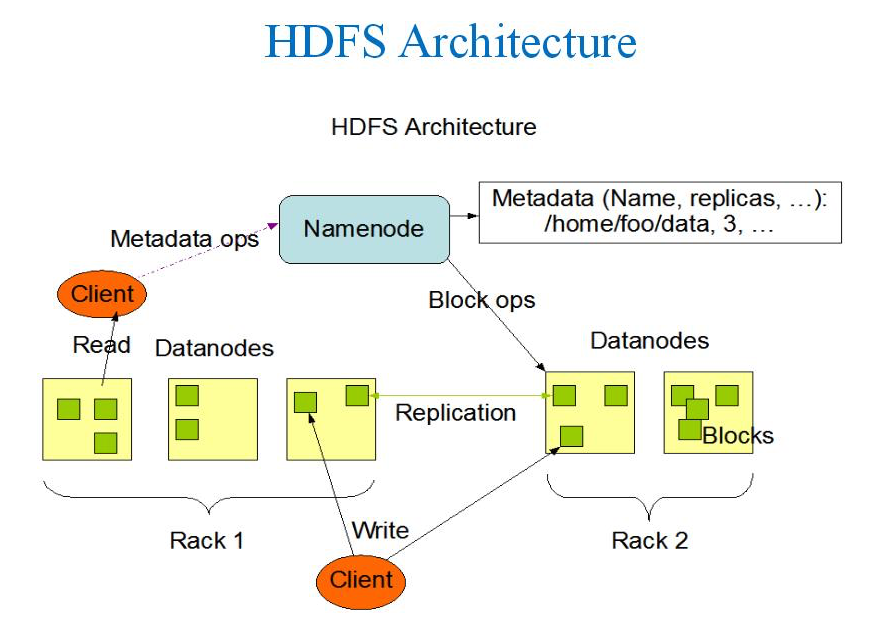
\includegraphics[width=10cm,height=7cm]{images/hdfs3}
\end{figure}

\newpage
\section{Ceph }

There are several SDS solutions available today. These include Ceph, GlusterFS, VMWare Virtual SAN and many more. Of these, Ceph is the most popular open source storage solution and hence we shall be looking at its architecture here.

There are three main components in the Ceph file system\cite{weil2006ceph} -- the client is one which exposes a POSIX style file interface to a host or process to interact with the Ceph cluster, a cluster of OSDs (Object Storage Devices) which are responsible for collectively storing object and object meta-data; and a cluster of meta data servers which manage namespace operations along with coordinating security, consistency and coherence.

Ceph architecture goals, as specified in the thesis describing ceph, include scalability to hundreds of peta bytes, performance and reliability. Unlike hadoop which is designed only for applications having a special type of workload i.e. single write multiple read, ceph allows more a general interface and includes capability of thousands of hosts concurrently reading and writing to the same file.


\begin{figure}[!htb]
\centering
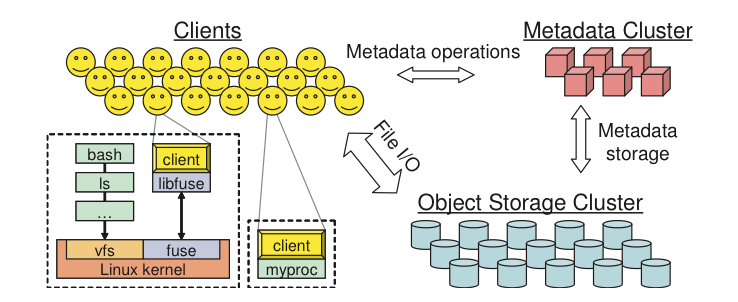
\includegraphics[width=11cm,height=7cm]{images/cepharch}
\caption[Long caption]{Architecture of Ceph Filesystem }
\end{figure}

Ceph  addresses the issue of scalability along with achieving high performance, reliability and availability through the following fundamental design features: decoupled data and metadata, dynamic distributed metadata management, and reliable autonomic distributed object storage. 

\begin{adjustwidth}{1.5em}{0pt}
\subsection{Decoupled Data and Metadata}
Just like Hadoop, Ceph also separates the concern of file system metadata management which includes file opening, renaming, moving etc from the storage of object data. The meta data operations are performed by the cluster of meta data servers whereas clients interact with the OSDs for I/O operations. Further as the storage devices operate directly on objects, low level block allocation decisions are delegated to the individual devices itself.
\end{adjustwidth}

\begin{adjustwidth}{1.5em}{0pt}
\subsection{Dynamic Distributed Metadata Management}
Ceph utilizes a novel meta data cluster architecture based on dynamic subtree partitioning\cite{weil2004dynamic}. Such a system adaptively and intelligently distributes the responsibility for managing the file system hierarchy among the multiple nodes present in the meta data cluster. The workload distribution among the meta data servers depends upon current access patterns while preserving the locality in each nodes workload and facilitating efficient updates and aggressive prefetching. This allows Ceph to scale meta data performance nearly linearly with the number of nodes in the meta data cluster.

\end{adjustwidth}

\begin{adjustwidth}{1.5em}{0pt}
\subsection{CRUSH}
    CRUSH stands for controlled replication under scalable hashing. Essentially it is a replacement for allocation lists, used by systems to find where the object is stored. Ceph Clients and Ceph OSD Daemons both use the CRUSH\cite{crush} algorithm to efficiently compute information about object location, instead of having to depend on a central lookup table. CRUSH provides a better data management mechanism compared to older approaches, and enables massive scale by cleanly distributing the work to all the clients and OSD daemons in the cluster. CRUSH uses intelligent data replication to ensure resiliency, which is better suited to hyper-scale storage. 
\end{adjustwidth}

\begin{figure}[!htb]
\centering
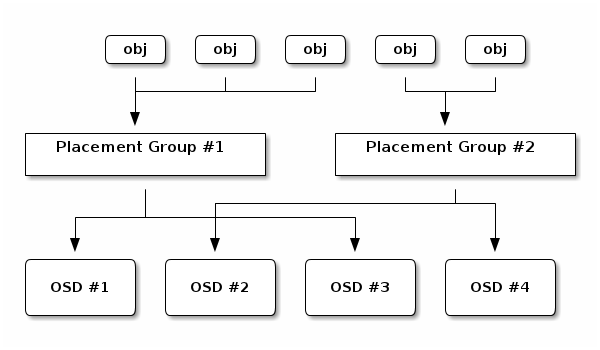
\includegraphics[width=10cm,height=7cm]{images/crush}
\caption[Long caption]{Assignment of osds to placement group is done using \emph{CRUSH} }
\end{figure}


\begin{adjustwidth}{1.5em}{0pt}
\subsection{RADOS}
    RADOS\cite{weil2007rados} refers to reliable autonomic distributed object storage. Large systems consisting of thousands of devices are dynamic in nature: they are built incrementally; grow and contract as new storage is added and old storage is decommissioned; device failures are frequent and expected; and large volumes of data are created, moved, and deleted. These factors require that the distribution of data evolve to effectively utilize available resources and maintain the desired level of data replication. In ceph the  responsibility for data migration, replication, failure detection, and failure recovery is delegated to the cluster of OSDs that is storing the data. Thus OSDs collectively appear to provide a single distributed and reliable object store to both clients and metadata servers.

\end{adjustwidth}

\begin{adjustwidth}{1.5em}{0pt}
\subsection{\small{High Availability Monitors}}
    Before Ceph Clients can read or write data, they must contact a Ceph Monitor to obtain the most recent copy of the cluster map. A Ceph Storage Cluster can operate with a single monitor; however, this introduces a single point of failure (i.e., if the monitor goes down, Ceph Clients cannot read or write data). So for added reliability and fault tolerance, Ceph supports a cluster of monitors. 
\end{adjustwidth}

\begin{figure}[!htb]
\centering
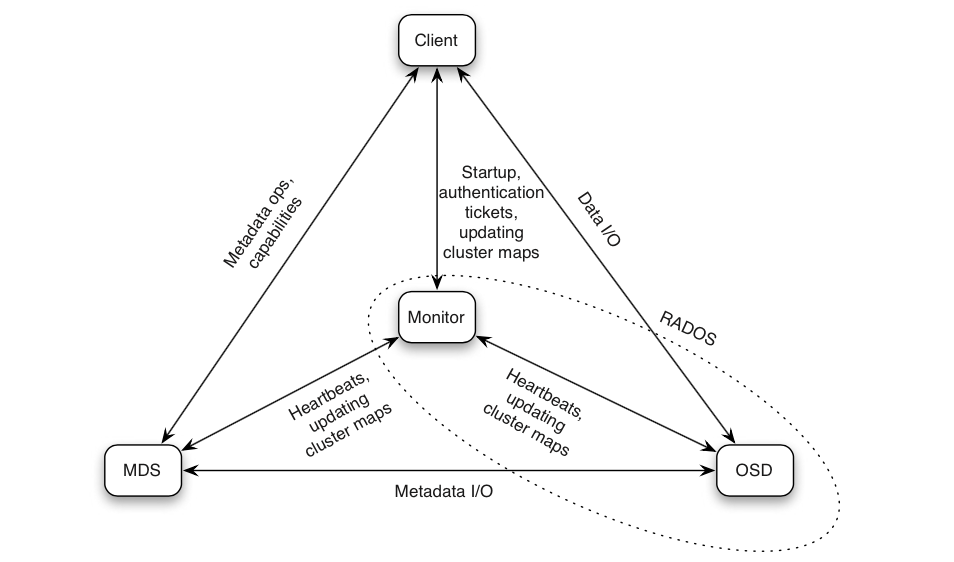
\includegraphics[width=10cm,height=7cm]{images/cephinter}
\caption[Long caption]{Ceph Component Interactions, highlighting the role of monitors }
\end{figure}



\newpage
\section{Comparison}
    Ceph has a number of features which make it very attractive for the massive growth in data in recent years (also referred to as big data). It has been designed for scalability, reliability, and performance. At the same time it assumes that failure of hardware is common, so it has been designed to adapt to these situations. Ceph breaks the file system into two pieces: (1) metadata, and (2) data. Separation of concerns allows ceph to implement an efficient and clean design for both parts.\cite{lwn}

    Ceph uses a dynamic distributed metadata server (MDS) that is not only clustered but also adapts to the changing workload. It will automatically distribute portions of the hierarchical directory tree to other MDS servers in the cluster to better load balance as the workload changes. In addition, if a MDS server is added, it will move portions of the metadata to that new box, again, improving the load distribution.
    
    Ceph's popularity is however nowhere close to that of the Hadoop file-system. Hadoop has only one metadata server and if it goes down entire system goes down. So it has only single point of failure and difficult to scale due to centralization of mds. Further object storage is not baked into the architecture of hadoop unlike ceph. Where hadoop wins out is the eco-system around it. Being widely popular it is already in use by several large organizations and has several additional components and layers on top of it. Numerous research papers around hadoop are available and even jobs are readily available. Despite being around for a long time ceph is yet to reach 1.0 and jobs are scarce. However having the solid foundation that it has the ceph may dominate the future.

\newpage
\section{Implementation}
\subsection{Virtual Environment}

    Here we shall briefly describe our efforts to set up a virtual ceph cluster. The setup involved four virtual machines (minimum) running on two physical machines. The virtualization software used was virtual box and the operating system on the virtual machines was ubuntu 14.04. Note that the space available for each vm (especially those which are to be used as OSDs later) must be greater than 30GB. Initial attempts to use another lighter virtualization software namely lxc were not successful as lxc shares/uses the host operating systems kernel and attempts to mount some modules which is not allowed in lxc. To allow the storage to be used as a service we decided to use a bridged network in virtual box.


    The process of setting up the cluster is straightforward. Using the ceph-deploy tool ceph was installed on one of the nodes. One of the nodes was used for administrating the cluster and hence referred to as admin-node. As host name resolution service was not accessible, the /etc/hosts file was edited to allow local resolution. The ceph cluster was then installed on each node using the ceph-deploy tool. Details of the installation and scripts to automate the process are available.
    
    After installing the ceph cluster, data was aggregated and block device simulated over it. This block device on another node referred to as client node (not a part of the cluster) which could then use it. The ext3 file system was configured over the block device and mounted in the userspace of the client node. It could then be used as additional file storage resource.

\subsection{General Computing Lab}    
    The next logical step would be to attempt to set-up a physical cluster comprising several nodes and test if it can be reliably used as a file-system for needs of the department. The department currently uses a proprietary solution by Netapp. This storage is proving to be expensive as it requires dedicated hardware to function. Using ceph on the large number of unused commodity hardware available with the department may be a viable option.
    
    We demonstrated by setting up a small 4 node cluster in department lab. The procedure was mostly similar barring a few exceptions. Firstly here the ceph process was operating on physical hardware. Further Internet access is not available for application installation on nodes of the lab. So we had to collect the packages and write a few scripts to make the installation procedure simpler. Finally after a few operational problems we were successful in pooling the hardware of the machines available and offering it as a resource to external nodes.
    
    While the cluster we set up was a small one comprising of four nodes, the department is considering the possibility of setting up a large cluster. Several uses can be envisioned of the extra storage that will be available such as serving as a secondary shared storage resource for the department and as a source of block devices for the Baadal VM. 
    

    

\section{Further Work}

Although we have demonstrated that Ceph can be useful for the department, before integrating the ceph file system, it is essential to validate its performance characteristics under a variety of workloads. Further there is a need to set up a system such that block storage can be acquired on demand by certain authorized applications. Such an infrastructure could serve as an extremely useful service for cloud systems such as the in house Baadal cloud.


\newpage
\medskip

\bibliographystyle{unsrt}%Used BibTeX style is unsrt
\bibliography{sample}

\end{document}
